\chapter{Approach}

\label{Chapter3}

\lhead{Chapter 3. \emph{Approach}}

\section{System overview} % (fold)
\label{sec:system_overview}

% section system_overview (end)

\section{Data ingestion and preprocessing} % (fold)
\label{sec:data_ingestion_and_preprocessing}

\begin{figure}[h]
  \centering
    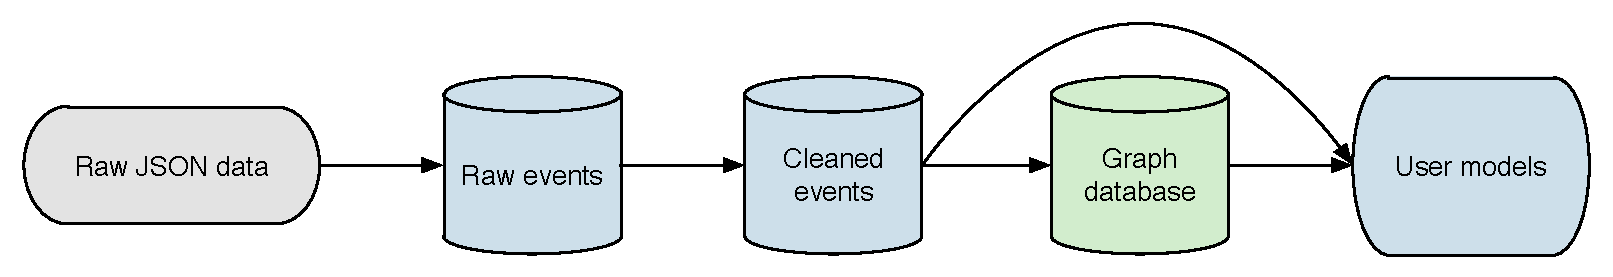
\includegraphics[width=\textwidth]{Figures/ingestion-pipeline}
  \caption{The ingestion pipeline broken into 4 steps. The color of each node indicates means of storage.}
  \label{fig:ingestion-pipeline}
\end{figure}

\emph{Blue} indicates a RDBMS, \emph{green} indicates a graph database, whereas \emph{gray} is used to indicate flat file storage.

% section data_ingestion_and_preprocessing (end)

\section{User modeling and clustering} % (fold)
\label{sec:user_modeling_and_clustering}

% section user_modeling_and_clustering (end)

\section{Adaptation component} % (fold)
\label{sec:adaptation_component}

\subsection{Evaluation metrics} % (fold)
\label{sub:evaluation_metrics}

\subsubsection{How to measure a positive user experience} % (fold)

% section evaluation_metrics (end)

\subsection{Applying the personalized feature set} % (fold)
\label{sub:applying_the_personalized_feature_set}

Description of the FlagService model.

% section applying_the_personalized_feature_set (end)

\subsection{Tracking user treatments} % (fold)
\label{sub:tracking_user_treatments}

% section tracking_user_treatments (end)

\subsection{Visualizing effects} % (fold)
\label{sub:visualizing_effects}

% section visualizing_effects (end)

% section adaptation_component (end)

\subsection{Differentiating product features} % (fold)
\label{sec:differentiating_product_features}

% section differentiating_product_features (end)

\section{Evolving the user models} % (fold)
\label{sec:evolving_the_user_models}

\subsection{Multi-arm bandits}

\subsection{Tracking individual treatment}

% section evolving_the_user_models (end)

\section{Visualization requirements (?)} % (fold)
\label{sec:visualization_requirements}

% section visualization_requirements (end)
